% DELIMITAÇÃO DO TEMA-------------------------------------------------------------------

\chapter{FUNDAMENTAÇÃO TEORICA}
\label{chap:delimitacao}

Neste capítulo serão apresentados conceitos fundamentais para o trabalho, permitindo que os leitores entendam de fato o como esse sistema foi desenvolvido e quais são as melhorias possíveis.\\
\\
Dessa forma, procura-se responder aos seguintes questionamentos:\\
O que é o ramo da computação?\\
O que é o GIT?\\
O que é o GITHUB?\\ 
O que é UIX e Experiencia do usuário?\\ 
O que é o HMTL?\\
O que é o CSS?\\
O que é a lógica de programação?\\ 
O que é um algoritmo?\\
O que é o JavaScript Vanilla?\\
O que é Phyton?\\
O que é aprendizado de máquina?\\
O que é uma Rede Neural?\\
O que é o GPT-3? 

\section{O ramo da computação e seus desafios.}
\label{sec:RamoComputacaoDesafios}
Em termos gerais, a computação pode ser definida como uma atividade realizada para processar as informações por meio de computadores. Esta atividade inclui o desenvolvimento de software e hardware também.

A utilização da tecnologia de computador para completar a tarefa é conhecida como computação.

Em um sentido moderno, usamos computadores para uma infinidade de finalidades - uma das quais é a crescente variedade de opções de entretenimento. No entanto, o hardware de computação moderno foi desenvolvido a partir de aparelhos muito maiores e muito mais básicos, nascidos principalmente da necessidade. O dispositivo computacional original era o ábaco, que foi supostamente inventado na antiga Babilônia por volta de 2.300 a.C. Algum tempo depois (por volta de 100 a.C.), o mecanismo de Antikythera foi usado para prever movimentos astronômicos com décadas de antecedência. Leia mais sobre a história da computação - Uma breve história da computação. 

\cite{whocomputing}

É com isto que lida a teoria da computação, subcampo da ciência da computação e da matemática. 

\section{O GIT}
\label{sec:OGIT}

	\subsection{VANTAGENS DE USAR O GIT}
	\label{sec:VANTAGENSGIT}

		Imagine que você esteja escrevendo um texto importante, escrevendo e apagando várias e várias vezes. Agora imagine que você tenha alterado seu texto demais e queira que ele volte a ser o que era antes, então você queria ter uma máquina do tempo, como a \textbf{TARDIS} da série cientifica \textbf{Doctor Who} e com ela você possa viajar no tempo e reescrever o texto a um ponto do passado. Isso é o que o \textbf{GIT} tenta fazer, ou seja, da mesma forma que a Tardis, ele grava todas as alterações dos arquivos de texto rastreados por ele, sendo possível realizar “\textbf{Commits}” que nada mais é que marcos dessas alterações, como se fosse uma data importante que algo relevante aconteceu, sendo possível voltar a esse ponto depois. 		

\begin{figure}
	\subsection{CONTROLE DE VERSÃO COM O GIT}
	\label{sec:CONTROLEVERSAOGIT}

	\centering
	\caption{Ilustração de o funcionamento do versionamento}
	\centering
	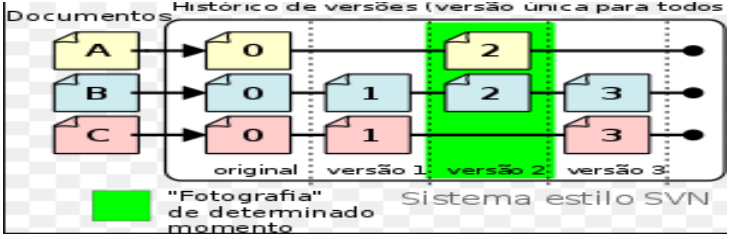
\includegraphics[scale=0.75]{./images/Figure_1}	
	
	\label{fig:Fig1}
\end{figure}

O \textbf{GIT} é um sistema de controle de versão distribuído gratuitamente e de código aberto. Escrito para gerenciar o
desenvolvimento do sistema operacional \textbf{Linux} de código aberto,
ele permite que grandes equipes de programadores trabalhem de
forma independente em suas próprias cópias do código, rastreiem
alterações com granularidade linha por linha, mesclem essas
alterações de volta no repositório principal e reverta as 
alterações conforme o necessário. \cite{whygit} 	

Para utiliza-lo, deve-se criar um repositório, clonar esse repositório e dar um \textbf{pull} (puxar) e fazer suas alterações no arquivo, devendo-se fazer um \textbf{commit} dessas alterações para marcar um revisão, depois de realizar todos os \textbf{commits} necessários com todas as revisões necessárias o usuário deve fazer o \textbf{push} (enviar) para o repositório para que as alterações e revisões vá para o repositório.\cite{githow} 

Para tanto, conta-se com a ajuda de um programa com uma interface visual de controle de versão (também conhecido como controle de revisão), o \textbf{scv} (sistema de controle de versão). ele mostra as linhas adicionadas com um destaque em verde e as linhas removidas com um destaque em vermelho, caso altere uma linha já existente ele coloca consecutivamente a remoção da linha antiga e a adição da linha nova. \cite{sourcetree}				

Vantagens de usá-lo: 
\begin{description}
	\setlength\itemindent{15pt}	
	\item[•] Trata-se de um sistema de controle de versão distribuído com um repositório do GitHub e cópias locais nas máquinas. Dessa forma, torna-se possível trabalhar com o projeto simultaneamente com outro profissional. 
	
	\item[•] Será possível saber o que foi modificado em cada revisão e, desa forma, possibilita visualizar a evolução do projeto e diagnosticar bugs mais facilmente ou desfazer as alterações que ocasionaram o erro. 
	
	\item[•] Refazer parte do código de modo correto, eliminando os erros anteriormente citados. 
	
	\item[•] Saber quem realizou as alterações, bem como sugerir a correção necessária. 
	
	\item[•] Em situações que dois programadores alterem o mesmo arquivo o sistema de controle de versão junta essas alterações através do merge e, caso alterem a mesma linha, o programador informa a ferramenta apropriada qual a linha correta. \cite{GitConflict}
	
\end{description}  	

\begin{figure}
	\centering
	\caption{Imagem do SourceTree em execução}
	\centering
	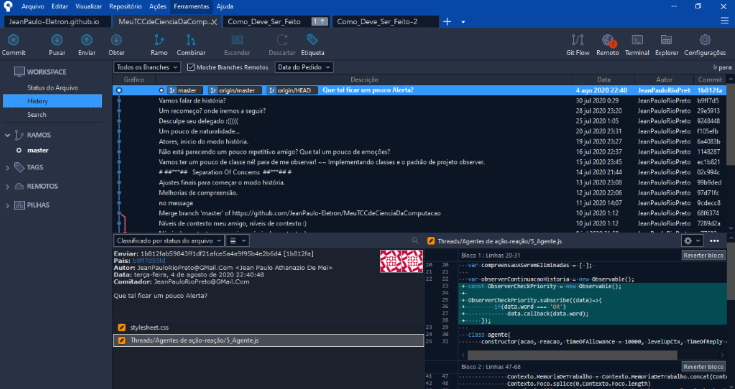
\includegraphics[scale=0.9]{./images/Figure_2}	
	
	Para este TCC o SourceTree foi o principal programa utilizado para o versionamento, juntamente com o GITHUB DESKTOP.	
	
	\label{fig:Fig2}
\end{figure}

\section{O GITHUB}
\label{OGitHub}

O \textbf{GitHub} é uma plataforma que fornece repositórios para armazenar arquivos e alterações nesses arquivos:\\ 
Muitos projetos \textbf{Open Source} foram criados a partir dele e, com esses projetos, os programadores podem contribuir para a comunidade e ainda ter visibilidade para o mercado, já que muitas empresas procuram programadores através de seus projetos no \textbf{GitHub} e suas contribuições em projetos \textbf{Open Source}. 

\begin{figure}[H]
	\centering
	\caption{Imagem do GITHUB}
	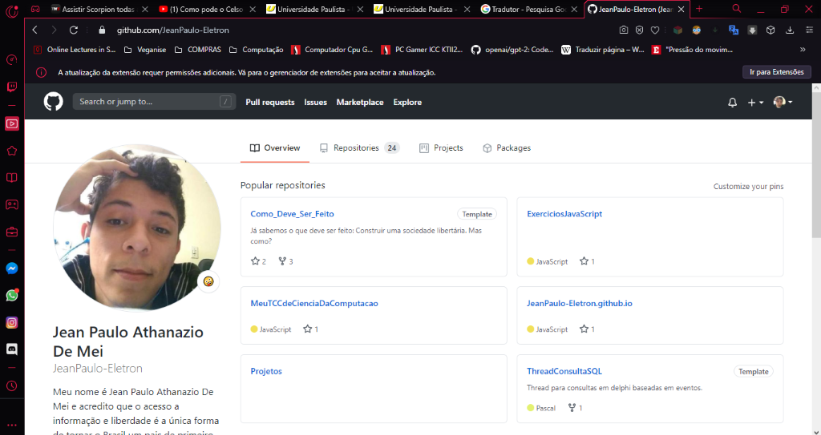
\includegraphics[scale=0.75]{./images/Figure_3}		
	\label{fig:Fig3}
\end{figure}

	\subsection{README}
	\label{subsec:README}
		É um arquivo que é exibido seu conteúdo de forma sumária ao entrar no repositório.

	
\section{EXPERIÊNCIA DO USUÁRIO}
\label{sec:EXPERIENCIADOUSUARIO}

	Experiência do usuário (UX), trata da interação do usuário com um
	determinado produto, sistema ou serviço cujo resultado gera uma
	percepção positiva ou negativa. Segundo Norman, UX envolve não somente
	aspectos relacionados ao design (hardware, software, interface,
	usabilidade, facilidade de busca etc), mas também destaca os aspectos
	afetivos e experienciais, significativos e valiosos de interação
	humano-computador e propriedade do produto. A experiência do usuário é
	de natureza subjetiva, pois é sobre a percepção e pensamento individual
	no que diz respeito ao sistema. Ela é também dinâmica, pois é
	constantemente modificada ao longo do tempo, devido à evolução das
	circunstâncias e inovações. (citação)
	
	Um conceito importante no design UX como os usuários formam
	experiências. Quando o usuário encontra um produto, forma uma impressão
	momentânea, que evolui ao longo do tempo. (citação)
	
	Neste processo, a percepção, ação, motivação e cognição do usuário se
	integram para formar uma história memorável: chamada “experiência do
	usuário”. Esse processo provoca respostas emocionais, que determinam em
	grande parte se a experiência será considerada positiva ou negativa.
	(citação) 

\section{HTML}
\label{sec:HTML}
	Antes de falar sobre HTML será necessário trazer à tona o conceito de camadas de desenvolvimento:
	\subsection{CAMADAS DE DESENVOLVIMENTO}
	\label{sec:CAMADASDEDESENVOLVIMENTO}
	
	\begin{figure}[H]
		\centering
		\caption{Imagem do SourceTree em execução}
		\centering
		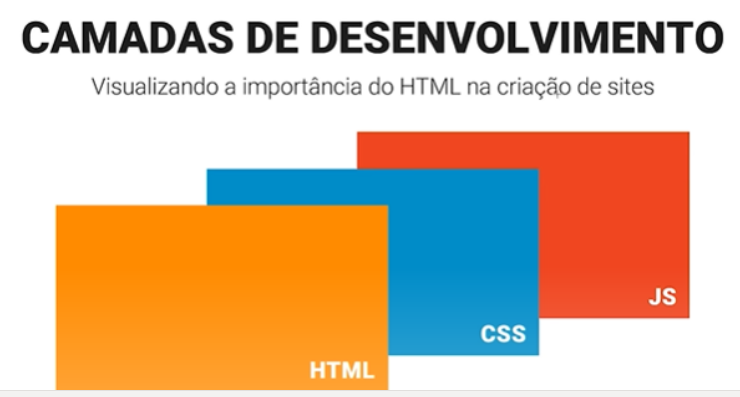
\includegraphics[scale=0.9]{./images/Figure_4}	
		
		Para este TCC decidi utilizar o SourceTree.	
		
		\label{fig:Fig4}
	\end{figure}
	\begin{description} 
		\item[Separation of concerns(Separação de conceitos):]
			antes de explicar o que são as camadas de desenvolvimento é importante conhecer o conceito de “separação de conceitos”, ela se refere a um princípio de projeto que permite a separação de um sistema em diferentes módulos. ao se combinar esses módulos tem-se o software, que pode ser uma página da web um hardware ou softwares desktop. essa separação é fortemente recomendável quando o software envolve uma complexidade muito alta e atende diferentes departamentos em uma única solução, com diversas regras de negócio diferentes, como módulo contábil, financeiro, rh, custos, controle de estoque, vendas... se ele foi programado de modo desacoplado(ou seja a alteração no código de um módulo não influencia no outro), definimos o software como modularizado, já que é constituído de diferentes partes. cada módulo pode ser alocado para uma equipe diferente de desenvolvimento, capacitada nas respectivas regras de negócio. assim, além de facilitar a manutenção, cada módulo poderá ser atualizado independentemente dos outros módulos. o delphi, por exemplo, propicia a modularização do software através de arquivos bpl para simplificar a atualização. \cite{SeparationOfConcerns}\\\\	
			programadores web praticam a separação de conceitos indiretamente. para construir uma página, normalmente quatro linguagens são utilizadas, cada uma com um propósito em particular: (citação) 
			
			\begin{description}
				\setlength\itemindent{15pt}
				\item[•] {HTML}
				\item[•] {CSS}
				\item[•] {JAVASCRIPT}
				\item[•] {BACKEND(PHYTON)}
			\end{description}
				
			nas quais poderemos intitulá-las como agentes de “conceitos”.  
			o html, é utilizado para descrever, dar significado, organizar e formatar o conteúdo de uma página, ou seja cada item/objeto contido nela estará lá, uma analogia seria com uma receita de bolo, você escreve a ordem correta de cada um dos ingredientes serem colocados (na página), assim o navegador consegue construir o site, porém ele não consegue modificar propriedades de um elemento/objeto da página depois de criado, e também não consegue fornecer um estilo próprio aquele objeto, essas atribuições são dadas ao css e javascript. (citação)\\\\			
			a linguagem css, por sua vez, edita a apresentação do conteúdo gerado pela linguagem html, fornecendo estilos aos componentes/objetos da página através do seu nome(id) ou através do nome do grupo ao qual aquele objeto pertence(classe), ou seja deixar ela bonita visualmente, fazendo outra analogia seria como colocar uma roupagem em cima do objeto feito pelo html. (citação)\\\\			
			o javascript é empregado para executar scripts do lado do cliente, ou seja alterar como os objetos já existentes se comportam ou tem de propriedade e criar objetos novos ao longo do tempo, dar comportamento a página, comportando-se de forma assíncrona para alterar a exibição do conteúdo sem comunicação com o servidor. (o jquery, por exemplo, fornece funções ajax, que permitem a alteração de um componente da página sem a necessidade de recarregá-la). (citação)\\\\		
			o back-end (“retaguarda”) de uma página, é responsável por manipular informações do banco de dados e executar operações de tratamento e envio de informações, com um servidor central ou distribuído, no escopo desse trabalho serão feitas pela linguagem phyton. (citação)				
	\end{description} 	
	  
	\subsection{ESTRUTURA DO HTML5}
	\label{subsec:ESTRUTURAHTML5}
	
	html (abreviação para a expressão inglesa hypertext markup language, que significa linguagem de marcação de hipertexto) é uma linguagem de marcação utilizada na construção de páginas na web.  (citação) 
	
	documentos html podem ser interpretados por navegadores. a tecnologia é fruto da junção  entre os padrões hytime e sgml. (citação) 	
		
	importante trazer a definição de hytime, que segundo (citação),  é um padrão para a representação estruturada de hipermídia e conteúdo baseado em tempo.
	
	um documento é visto como um conjunto de eventos concorrentes dependentes de tempo (como áudio, vídeo, etc.), conectados por hiperligações (em inglês: hyperlink e link). o padrão é independente de outros padrões de processamento de texto em geral. 
	
	sgml é um padrão de formatação de textos. não foi desenvolvido para hipertexto, mas tornou-se  conveniente para transformar documentos em hiper-objetos e para descrever as ligações. 	
	
	marcas (tags): todo documento html possui marcadores (do inglês: tags), palavras entre parênteses angulares(símbolos de maior e de menor “>” “<”), esses marcadores são os comandos de formatação da linguagem. um elemento é formado por um nome de marcador (tag), atributos, valores e filhos (que podem ser outros elementos ou texto). os atributos modificam os resultados padrões dos elementos e os valores caracterizam essa mudança. exemplo de um elemento simples (não possui filhos): 
	
	\begin{verbatim}	
		<hr /> 
		Exemplo de um elemento composto (possui filhos): 
		
		<a href="http://pt.wikipedia.org/">Wikipédia</a> 	
	\end{verbatim}
	Exemplo de um código HTML:		
	\begin{figure}[H]
		\centering
		\caption{Imagem de um código HTML}
		\centering
		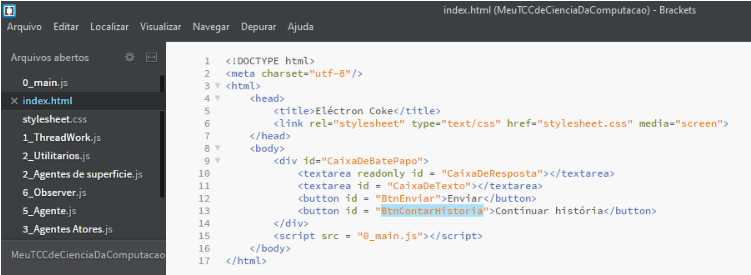
\includegraphics[scale=0.75]{./images/Figure_5}	
		\label{fig:Fig5} 
	\end{figure}	
	Esse código é um código HTML justamente desse TCC, uma versão mais antiga de 12/10/2020, mas que já dá uma ideia de como funciona o HTML.
	
\section{CSS}
\label{sec:CSS}

O QUE É CSS? Cascading Style Sheets (CSS) é um mecanismo simples para adicionar estilo (por exemplo, fontes, cores, espaçamento) a documentos da Web.6 

Desta forma é possível deixar o visual da página mais agradável visualmente, tendo uma identidade visual própria, sem ele todas as páginas seriam preto e branco, sem cores... 
Exemplo de um código CSS: 

\begin{figure}[H]
	\centering
	\caption{Imagem de um código CSS}
	\centering
	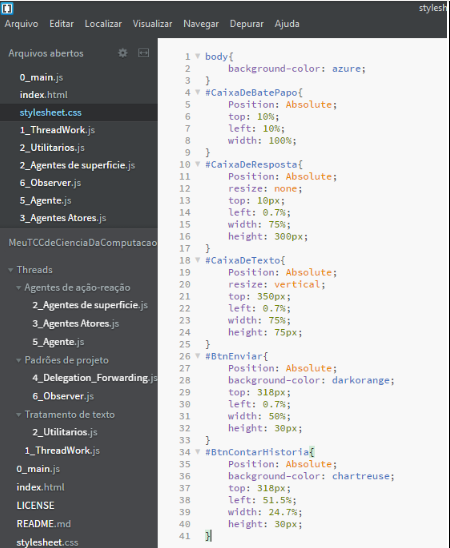
\includegraphics{./images/Figure_6}	
	\label{fig:Fig6} 
\end{figure}

\section{LÓGICA DE PROGRAMAÇÃO }
\label{sec:LÓGICA DE PROGRAMAÇÃO}

O computador não consegue interpretar diretamente um texto escrito em linguagem natural, devido as ambiguidades presente na nossa linguagem, então para que ele possa entender o que tem que ser feito é necessário escrever para ele o que tem que ser feito de forma muito didática, descrevendo com muitos detalhes.   

A lógica de programação envolve operações lógicas que são realizadas em dados concretos, elas funcionam a partir de princípios lógicos e o resultado da execução dos algoritmos(sequência de passos[que ele entende o significado] informados ao computador para que ele possa cumprir um determinado objetivo) feitos através dela podem ser quantificados. 

A distinção importante aqui é que a lógica de programação, e a lógica em geral, é fundamentalmente definida contra outros tipos de programação que não são construídos em lógica rígida ou estados e resultados quantificáveis. 

Por exemplo, a lógica modal por sua natureza é comparada às operações quânticas teóricas que não fornecem um estado de conjunto específico ao qual os computadores podem aplicar a lógica. 

A lógica de programação em geral repousa sobre uma base de lógica computacional que é compartilhada por humanos e máquinas, que é o que exploramos à medida que continuamos a interagir com novas tecnologias. Com isso em mente, pode-se desenvolver definições mais específicas de uma lógica de programação relacionada à base de um trecho de código. 

\section{ALGORITMOS}
\label{sec:ALGORITMOS}

Todo programador para conversar com o computador e dizer a ele o que fazer usa o “código”, mas para ele escrever e montar esse código é necessário conhecer o conceito de algoritmo.  

Um algoritmo pode ser definido como uma sequência de raciocínios, instruções ou operações para alcançar um objetivo, sendo necessário que os passos sejam finitos e operados sistematicamente. 
Ele é fundamental para o ramo da computação, é através dele que os sistemas são criados, possibilitando ter acesso a dados que antes não eram possíveis só no papel e caneta(por serem quantidades colossais de dados a serem analisados a mão), os algoritmos são geralmente criados de forma a ser independente de uma linguagem, ou seja, um mesmo algoritmo pode ser implementado em mais de uma linguagem de programação... 

Porém eles são muito importantes fora da computação, alguns exemplos de algoritmos que podemos citar são: receitas culinárias, manual de instrução de aparelhos e funções matemáticas. 

Uma receita culinária, por exemplo. Nela pode se encontrar os ingredientes necessários (dados de entrada), o passo a passo para realizar a receita (processamento ou instruções lógicas) e atinge um resultado (o prato finalizado). 
Um algoritmo, portanto, conta com a entrada (input) e saída (output) de informações mediadas pelas instruções, é fundamental compreender que o algoritmo se justifica no resultado que ele almeja alcançar, logo, deve ter um objetivo específico. Uma sequência de instruções simples pode se tornar mais complexa conforme a necessidade de considerar outras situações e se o algoritmo não for bem dimensionado em relação a quantidade e complexidade dos dados aos quais ele for exposto, ele pode travar ou não fornecer a resposta esperada, por conta disso, o algoritmo tende a crescer e ficar mais complexo com o passar do tempo para englobar todos os cenários possíveis. 
Ao montar a estrutura do algoritmo deve se ter em mente que para funcionar da forma esperada ele precisa seguir uma lógica sistemática. Por exemplo, se você está fazendo um bolo, mas “pula” a etapa de inserir farinha, no final, você não terá mais um bolo. 
Com o código, é a mesma coisa, sendo necessário ler linha por linha para que ele atinja o objetivo final. As estruturas de um algoritmo são: 

\begin{description}
	\setlength\itemindent{15pt}
	\item[•] variáveis: são as informações de entrada inseridas que determinam aonde o algoritmo poderá ir. As mais comuns são texto, inteiro, lógico e real; 
	\item[•] comandos de repetição: consiste no uso de “se” e “enquanto”, para que o algoritmo saiba o que fazer quando determinados processos ocorrerem e o que fazer se eles mudarem. 
\end{description}

\begin{figure}[H]
	\centering
	\caption{Exemplos de algoritmos}
	\centering
	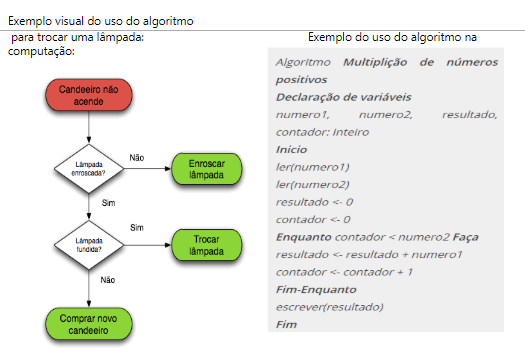
\includegraphics{./images/Figure_7}	
	\label{fig:Fig7}
	\centering
	\\Disponível em: https://dicasdeprogramacao.com.br/o-que-e-algoritmo/  
\end{figure}

\section{PHYTON}
\label{sec:PHYTON}
Essa será a linguagem utilizada no BackEnd, comumente usado para desenvolver algoritmos e aplicações de inteligência artificial. 

\section{INTELIGÊNCIA ARTIFICIAL}
\label{sec:inteligênciaartificial}

A Inteligência Artificial (IA) é um avanço tecnológico que permite que sistemas simulem uma inteligência similar à humana — indo além da programação de comandos específicos e bem definidos para tomar decisões de forma autônoma, baseadas em padrões de comportamento promissores obtidos através do refinamento de um algoritmo que varre enormes bancos de dados e métricas muito bem estipuladas do quão bom está esse comportamento. 

Há algumas décadas, se estuda os denominados “agentes inteligentes”, que percebem seu ambiente, entendem como podem operar e qual a melhor forma, essa foi a principal forma de inteligência computacional antes do novo milénio.

\section{REDES NEURAIS E APRENDIZADO DE MÁQUINA}
\label{sec:REDESNEURAISEAPRENDIZADODEMÁQUINA}

As redes neurais artificiais tem como objetivo emular o comportamento biológico do cérebro humano e nos processadores de um computador, o cérebro humano pode ser comparado a um computador altamente complexo, não linear e paralelo, por meio de seus neurônio ele consegue processar as informações (e realizar de forma muito mais rápida certas tarefas que um computador digital faz de forma satisfatória, como, reconhecimento de padrões, percepção, controle motor...), por tanto os algoritmos de Redes Neurais tem por objetivo emular “a aprendizagem”, ou seja interagir com o ambiente ao qual ele foi exposto, colocar métricas de desempenho reforçando os bons comportamentos e punindo os comportamentos ruins, alterando as conexões e pesos de sua rede neural com o intuito armazenar o comportamento adquirido e adquirir novos comportamentos que podem ser melhores...  
O procedimento usado para que a aplicação aprenda é chamado “algoritmo de aprendizagem”, entre seus pontos fortes estão o fato que a estrutura interna de uma rede neural é altamente distribuída e descentralizada, capacidade de ser linear e não linear (ao passar pelos pesos eles se encontram em um neurônio ao qual esses valores passam por uma função matemática de ativação, que pode ser linear ou não linear), é possível fazer o mapeamento da entrada e da saída, assim sendo é possível criar modelos estatísticos visando melhorar o comportamento da rede como um todo, além disso ela tem a capacidade de adaptar seus pesos para se comportar corretamente com as alterações do ambiente, se o ambiente for não estacionário(ou seja muda muito ao longo do tempo), a rede pode ser projetada para adequar seus pesos em tempo real com o objetivo de aumentar sua performance para novamente um nível satisfatório, ela pode também classificar o nível de crença na resposta dada, assim caso ela se encontrar com padrões ambíguos ela pode escolher qual entre eles é o mais próximo de sua crença de ser o padrão correto, pela sua forma de implementação com vários neurônios um afetando o outro a informação contextual também é armazenada, pelo fato de ter muitos neurônios ela também é tolerante a falhas de hardware, ela pode ser implementada de maneira hierárquica, a mesma notação matemática pode ser utilizado em todos os domínios de redes neurais, e também possuem uma analogia neurobiológica, se baseiam no sistema mais complexo e mais poderoso e tolerante a falhas que existe. 

\section{OPENAI, GPT-2 E GPT-3}
\label{sec:OPENAI}

OpenAI é uma instituição sem fins lucrativos de pesquisa em inteligência artificial, que tem como objetivo promover e desenvolver IA amigável, de tal forma a beneficiar a humanidade como um todo. 
O GPT-2 é uma IA de conversação em linguagem natural de código aberto, o GPT-3 é a evolução do GPT-2 por meio de uma API (disponível em: https://openai.com/blog/openai-api/). 
